
\pagebreak

\subsection{Carnot and Rankine Steam Cycles}


\begin{enumerate}

%%%
%%%
%%%
\item {\it In a turbine, steam at 20 bar, 360$^{o}$C is expanded to 0.08 bar. The steam is condensed into saturated liquid water. The pump feeds the water back into the boiler. Assume ideal processes, calculate the net work per kg of steam and the cycle efficiency.}\label{Example_01_01}

\begin{figure}[h]
\begin{center}
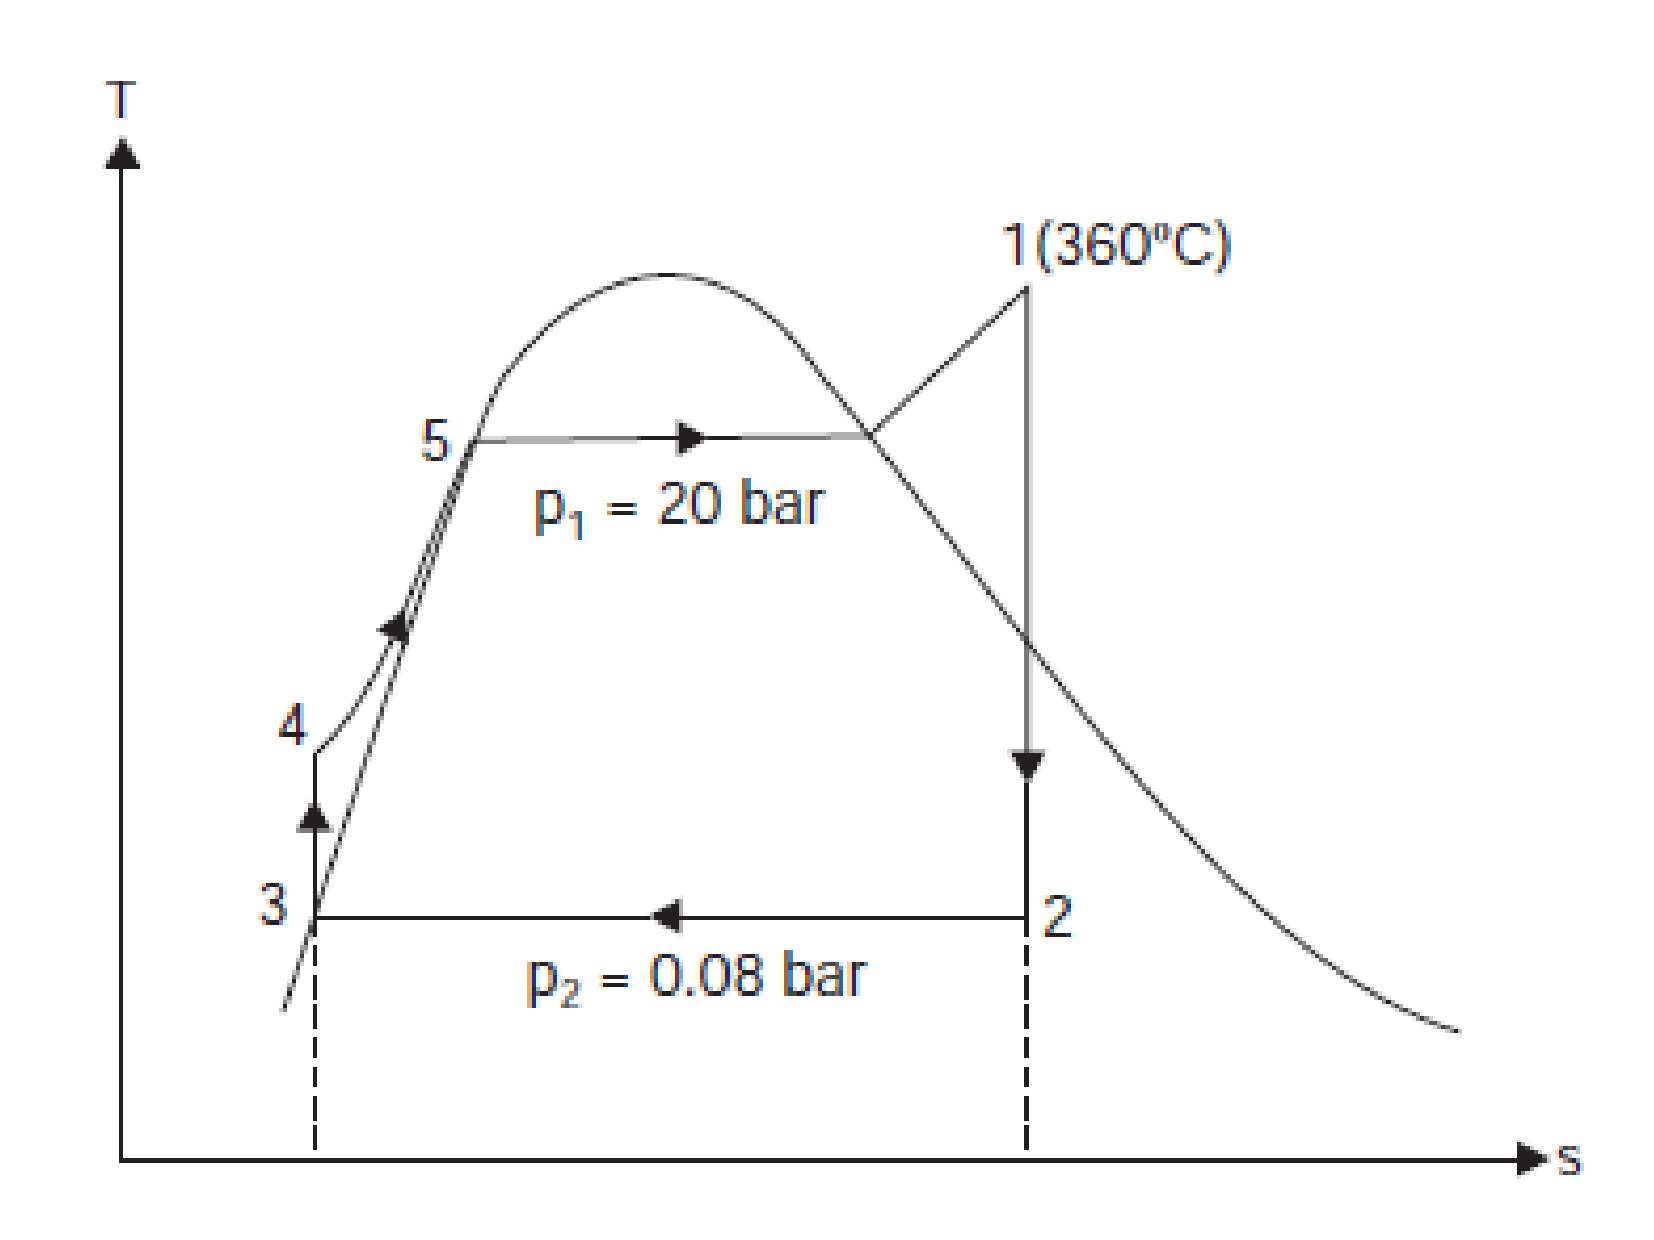
\includegraphics[width=13.0cm,height=8.0cm]{./Pics/example01_01}
\end{center}
\caption{Carnot and Rankine Cycles: Ts diagram -- Example \ref{Example_01_01}.}
\label{Example01_01:Pic1}
\end{figure}

As the process {\it 1-2} is isentropic (Fig. \ref{Example01_01:Pic1}), $s_{1}=s_{2}$ and using the data in Table \ref{Example01_01:Table1},
\begin{eqnarray}
&& 6.9917 = s_{f,2}+x_{2}s_{fg,2} = 0.5926 + 7.6361 x_{2} \;\; \Longrightarrow \;\; x_{2}= 0.838 \nonumber \\
&& h_{2} = h_{f,2}+ x_{2}h_{fg,2} \;\; \Longrightarrow h_{2}=2187.68\;kJ/kg \nonumber
\end{eqnarray}

\begin{center}
\begin{table}[h]
\begin{tabular}{c c c c c c c c c }
\hline
                    & $P$   & $T$ &  $h_{f}$  & $h_{fg}$ & $s_{f}$      & $s_{fg}$      & $s_{g}$        &   $v_{f}$ \\
                    & (bar) & (K) &  (kJ/kg) &  (kJ/kg) & (kJ/(kg.K)) & (kJ/(kg.K))   & (kJ/(kg.K))   &$\left(m^{3}/kg\right)$ \\
\hline
{\it Boiler}        & 20    & 633.15& 3159.3  & --      & 6.9917      & --            & --             & --  \\
\hline
{\it Condenser}     & 0.08  &  --  & 173.88  & 2403.1   & 0.5926      &  7.6361       & 8.2287         & 1.008$\times$10$^{-3}$ \\
\hline
\end{tabular}
\caption{Carnot and Rankine Cycles: Steam tables -- Example \ref{Example_01_01}.}
\label{Example01_01:Table1}
\end{table}
\end{center}

The net work $\left(W_{\text{net}}\right)$ is calculated from, $W_{\text{net}}=W_{\text{turbine}}-W_{\text{pump}}$. The work required by the pump is
\begin{eqnarray}
&& W_{\text{pump}}=h_{f,4}-h_{f,3}=v_{f,2}\left(P_{1}-P_{2}\right) = 1.008\times 10^{-3} \left[\frc{m^{3}}{kg}\right] \times (20-0.08) [bar] \times \left[\frc{100\;kJ/kg}{m^{3}.bar/kg}\right] = 2.008\; kJ/kg \nonumber \\
&& h_{f,4} = 2.008+h_{f,2}=175.89\;kJ/kg\nonumber
\end{eqnarray}
And the work produced by the tubine is defined as
\begin{displaymath}
W_{\text{turbine}}=h_{1}-h_{2} = 3159.3-2187.68= 971.62 \; kJ/kg
\end{displaymath}

And the net work is
\begin{eqnarray}
&& W_{\text{net}}=W_{\text{turbine}}-W_{\text{pump}} = 971.62-2.008 \nonumber \\
&& \textcolor{red}{W_{\text{net}}=969.61\frc{kJ}{kg}} \nonumber
\end{eqnarray}

The efficiency of the cycle is obtained by the relationship $\eta_{\text{cycle}}=\frc{W_{\text{net}}}{Q_{1}}$. The heat added into the boiler $\left(Q_{1}\right)$ is given by,
\begin{displaymath}
Q_{1}=h_{1}-h_{f,4}=3159.3-175.89=2983.41\;kJ/kg
\end{displaymath}
and the efficiency is
\begin{displaymath}
\textcolor{red}{\eta_{\text{cycle}}=\frc{969.61}{2983.41}=0.325\text{ or } 32.5\%}
\end{displaymath}


%%%
%%%
%%%
\item {\it A Rankine cycle operates between pressures of 80 and 0.1 bar and the maximum temperature is 873.15 K. Assuming that the steam turbine and condensate pump efficiencies are 90$\%$ and 80$\%$, respectively, calculate the specific work and thermal efficiency.}\label{Example_01_02}

From the saturated water and steam tables:

\begin{center}
\begin{table}[h]
\begin{tabular}{||c|c|c c|c c c|c c c||} 
\hline\hline
{\bf P (bar)} & {\bf T (K)} & \multicolumn{2}{|c|}{{\bf Specific Volume $\left(m^{3}/kg\right)$}} & \multicolumn{3}{|c|}{{\bf Specific Enthalpy (kJ/kg)}} & \multicolumn{3}{|c||}{{\bf Specific Entropy (kJ/(kg.K)}}  \\
\hline
              &             &  $v_{f}$                  &    $v_{g}$                              &  $h_{f}$    &  $h_{fg}$  &   $h_{g}$                 &  $s_{f}$  &  $s_{fg}$    &  $s_{g}$  \\
\hline\hline
0.1           & 318.99      &1.0103$\times$10$^{-3}$    & 0.1468$\times$10$^{2}$                  & 191.9   & 2392.3    & 2584.2              & 0.6488 & 7.5006  & 8.1494 \\
80            & 568.25      &1.385$\times$10$^{-3}$     & 0.0235                                  & 1317.0 & 1440.5   & 2757.5               & 3.2073 & 2.5351  & 5.7424  \\
\hline\hline
\end{tabular}
\caption{Carnot and Rankine Cycles: From Saturated water and steam tables.}
\label{Example01_01:Table2}
\end{table}
\end{center}


\begin{table}[h]
\begin{center}
\begin{tabular}{c c r}
\multicolumn{3}{c}{Superheated Steam} \\
\hline
\multirow{3}{*}{$P=80\;bar\;,\;T= 600^{o}C$} & $v$ & 0.486 m$^{3}$/kg \\
                           & $h$ & 3642 kJ/kg \\
                           & $s$ & 7.0206 kJ/(kg.K)\\
\hline
\end{tabular}
\end{center}
\caption{Carnot and Rankine Cycles: From Superheated Steam.}
\label{Example01_01:Table23}
\end{table}

Since $s_{1}=s_{2}$, the steam quality is calculated from,
\begin{eqnarray}
&& s_{2} = s_{f,2}+x_{2}s_{fg,2} \nonumber \\
&& 7.0206 =  0.6488 + 7.5006 x_{2} \nonumber \\
&& x_{2}= 0.85
\end{eqnarray}
and the enthalpy is obtained from 
\begin{displaymath}
h_{2}=h_{f,2}+x_{2}h_{fg,2} =191.9+0.85\times 2392.3 = 2225.36\; kJ/kg
\end{displaymath}
And the work


\begin{figure}[h]
\begin{center}
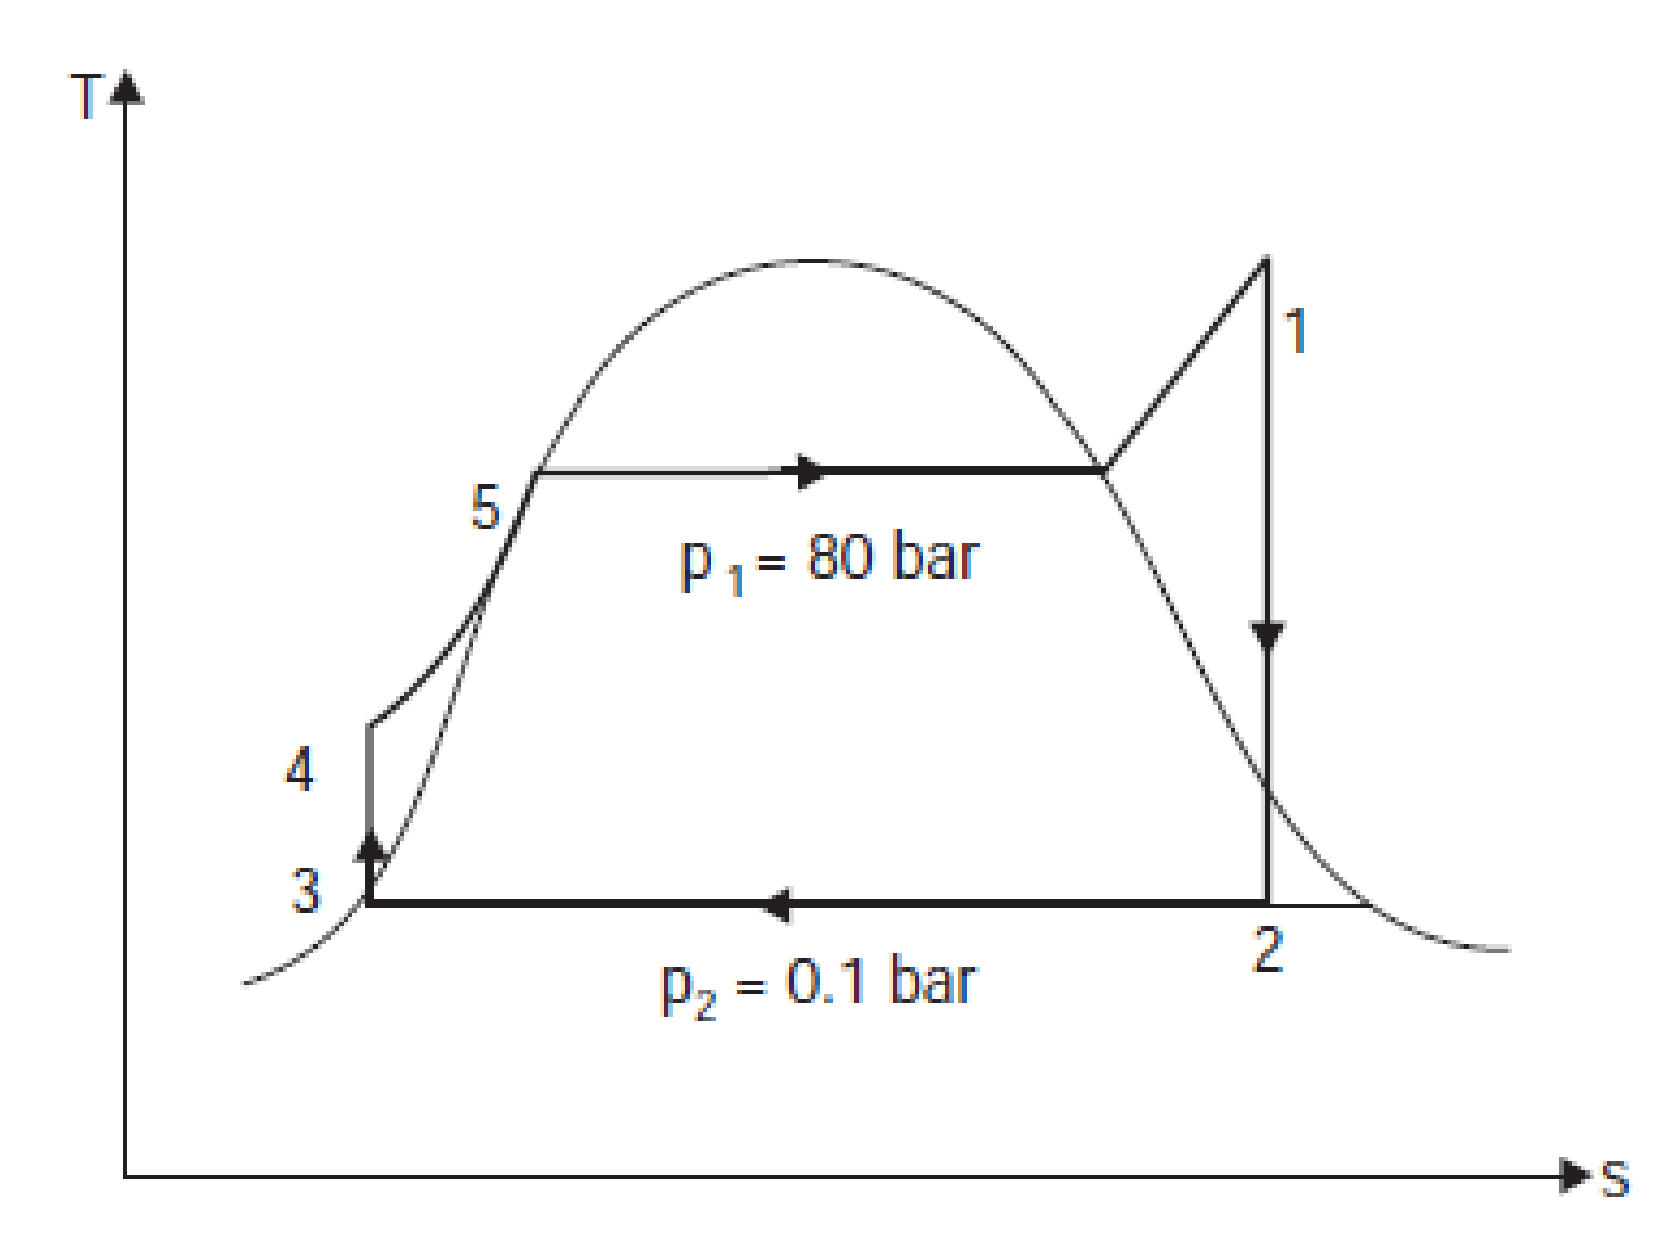
\includegraphics[width=13.0cm,height=8.0cm]{./Pics/example01_02}
\end{center}
\caption{Carnot and Rankine Cycles: Ts diagram -- Example \ref{Example_01_02}.}
\label{Example01_01:Pic2}
\end{figure}

%%%
%%%
%%%
\item {\it In a steam power plant operating on the Rankine cycle, steam enters the turbine at 30 bar and 623.15 K and later condensed at 0.1 bar. Calculate: (a) thermal efficiency; (b) thermal efficiency assuming that the steam is superheated to 873.15 K before entering the turbine; (c)thermal efficiency assuming that the boiler pressure is raised to 150 bar while the inlet temperature at turbine is maintained at  623.15 K.}\label{Example_01_03}


\begin{enumerate}
\item \label{example_01_03_a}The {\it Ts} diagrams of the cycle for all three cases can be seen in Fig. \ref{Example01_01:Pic3}, and the original phase states can assigned as 

\begin{tabular}{l l l l}
$P_{1}=0.1\;bar$ (saturated liquid) &  $P_{2}=30\;bar$ & $P_{3}=30\;bar$           & $P_{4}=0.1\;bar$ \\
$h_{1}=191.81\;kJ/kg$               &  $s_{2}=s_{1}$   & $T_{3}=623.15\;K$         & $s_{4}=s_{3}$ \\
$v_{1}=1.01\times 10^{-3}\;m^{3}/kg$ &                  & $h_{3}=3116.1\;kJ/kg$     &                 \\
                                    &                 & $s_{3}=6.7450\;kJ/(kg.K)$ &                 \\
\end{tabular}


\begin{figure}[h]
\begin{center}
\vbox{
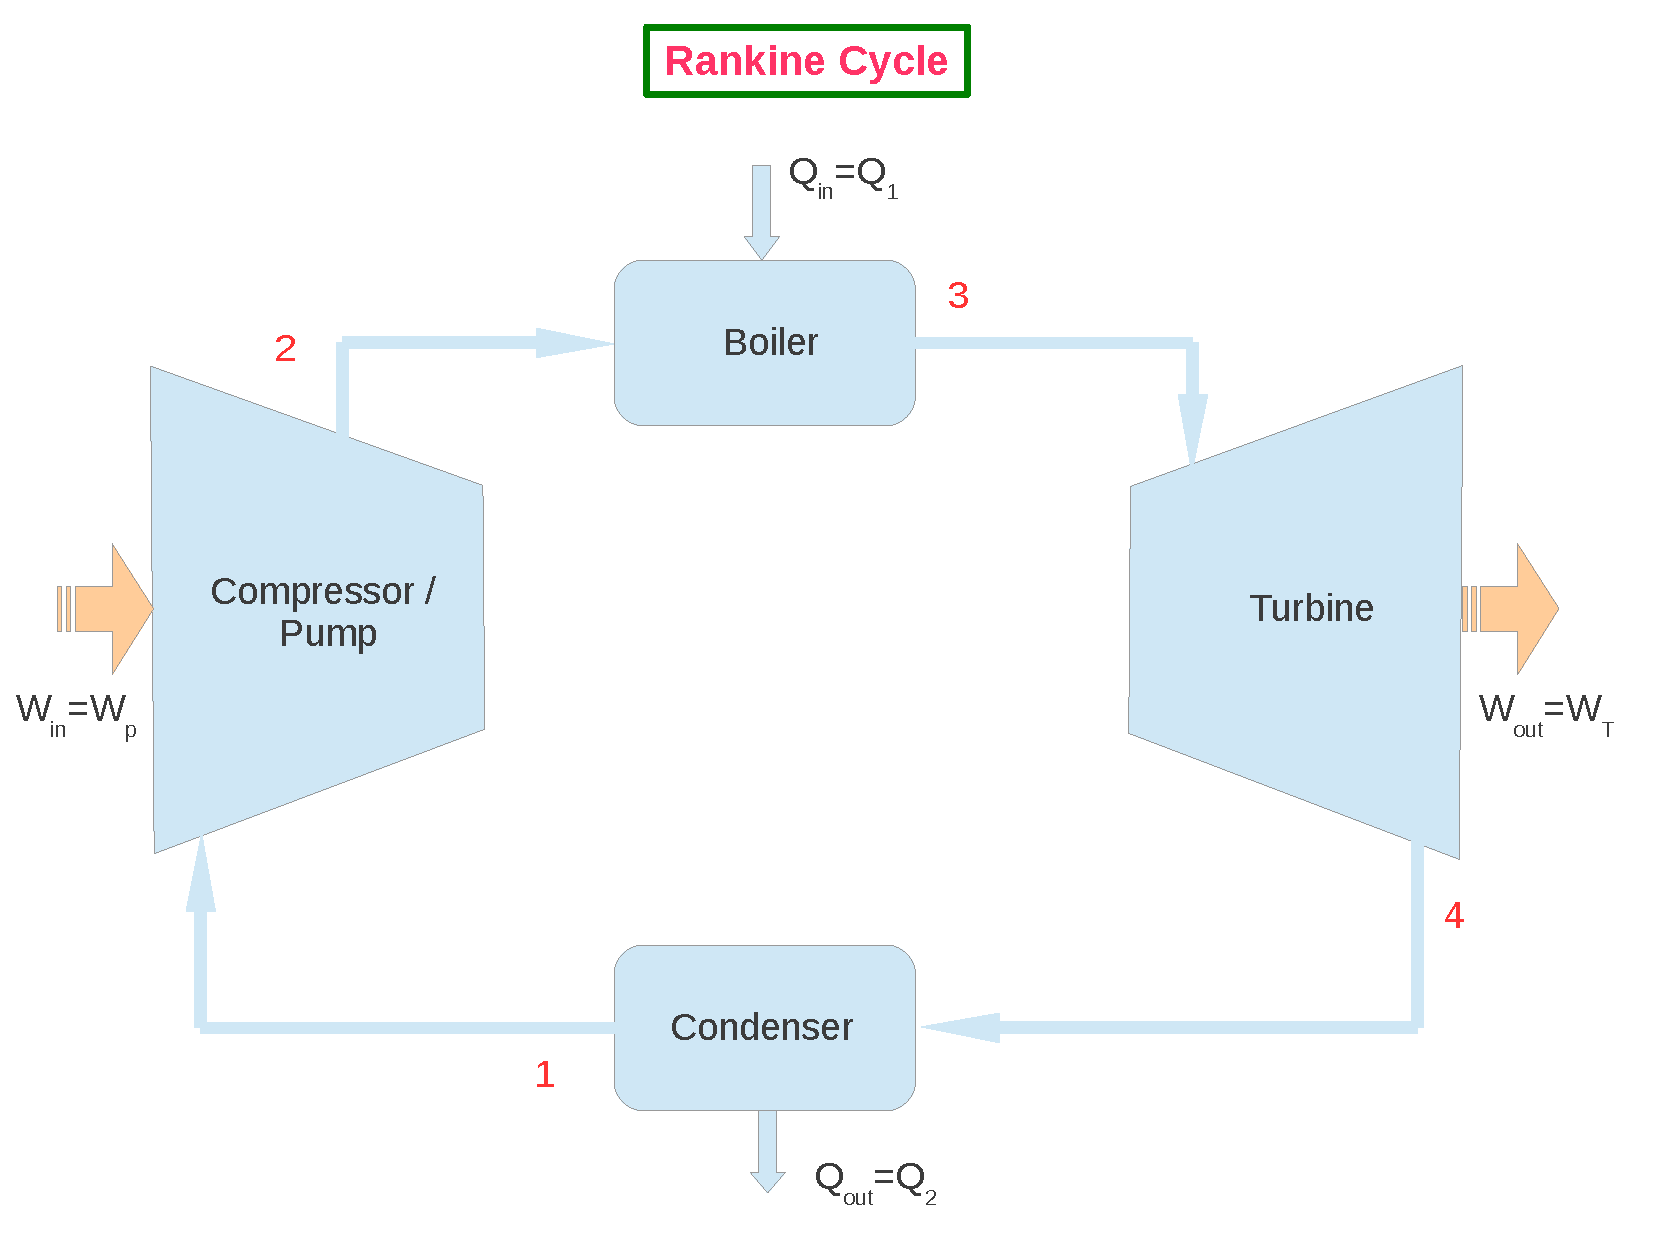
\includegraphics[width=13.0cm,height=9.0cm]{./Pics/Simple_Rankine_Cycle_2}
\vspace{-1.cm}
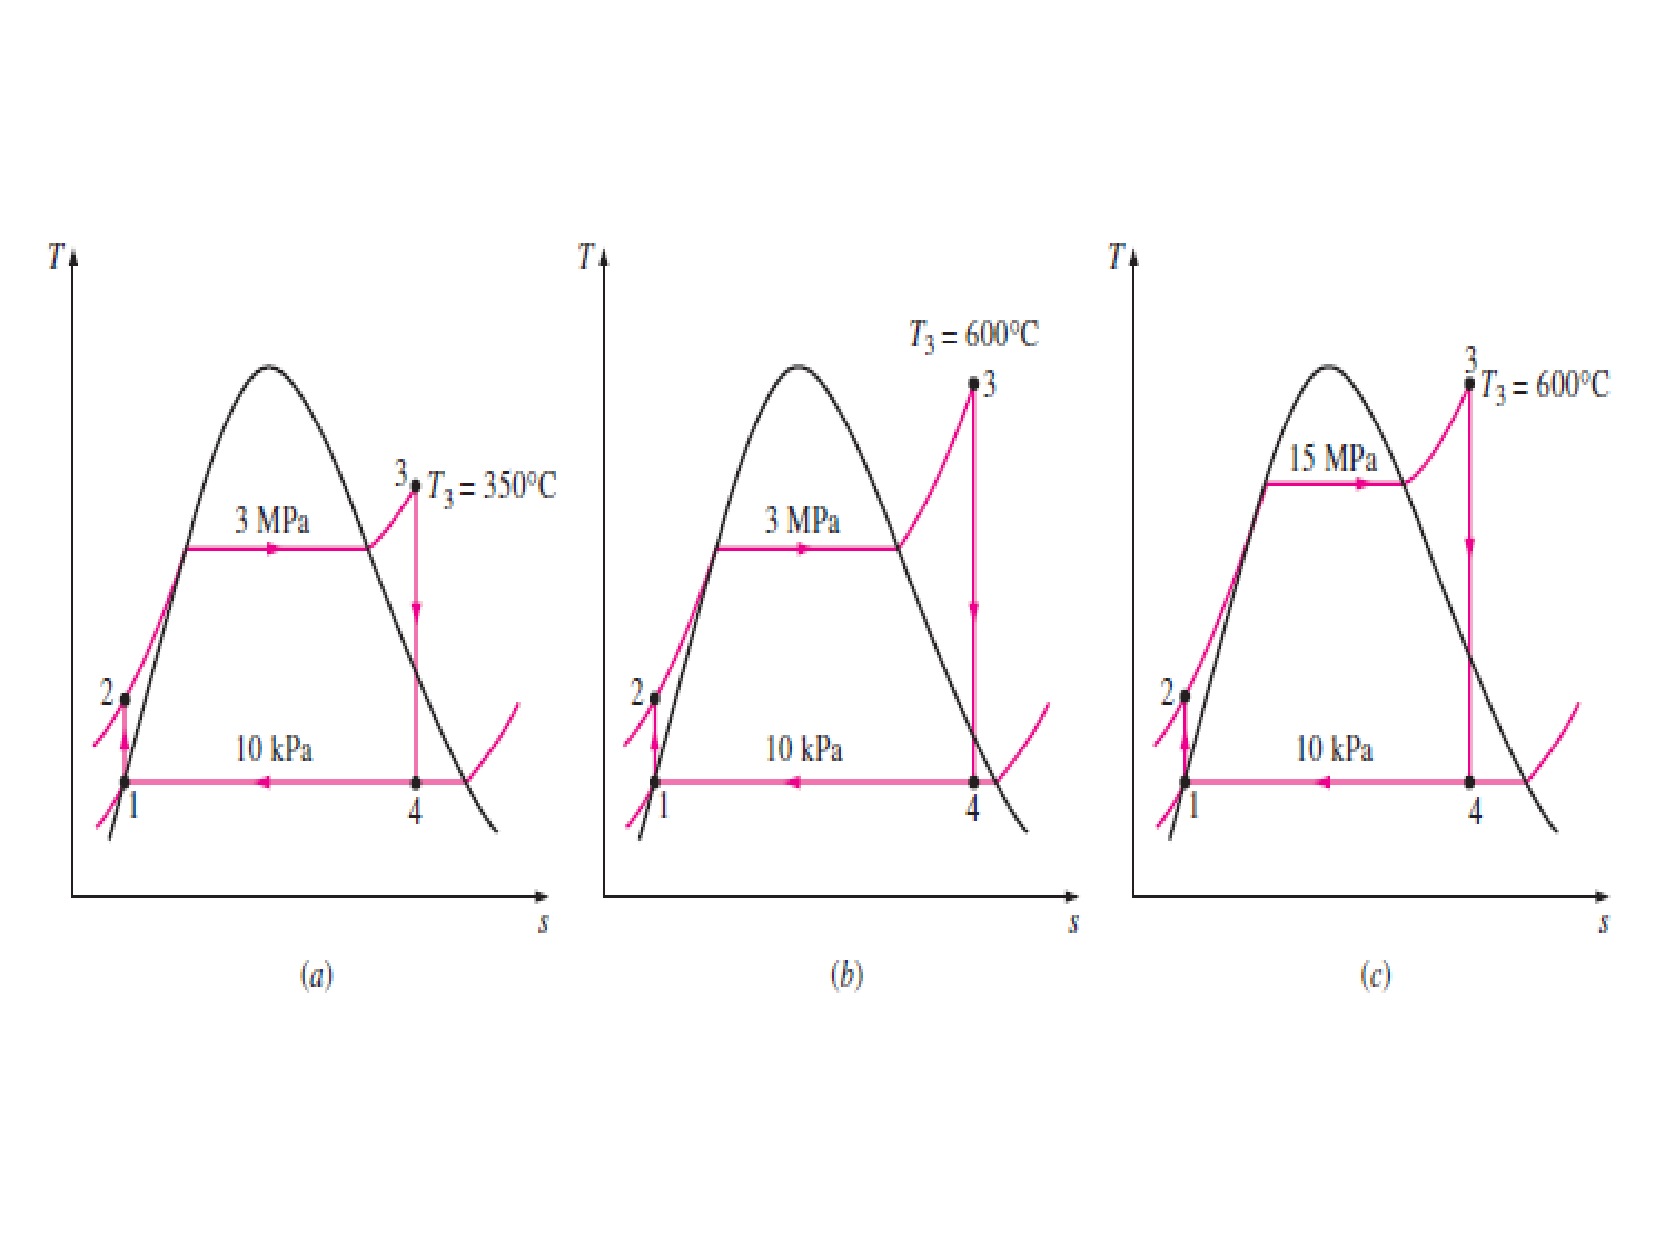
\includegraphics[width=15.0cm,height=9.0cm]{./Pics/example01_03}
}
\end{center}
\caption{Carnot and Rankine Cycles: Schematic of a Rankine cycle and Ts diagrams -- Example \ref{Example_01_03}.}
\label{Example01_01:Pic3}
\end{figure}

Enthalpy of the fluid leaving the pump can be calculated as
\begin{displaymath}
h_{2}=h_{1}+W_{\text{in}}
\end{displaymath}

where the pump work can be computed as
\begin{displaymath}
W_{\text{in}}=v_{1}\left(P_{2}-P_{1}\right)=3.02\;kJ/kg
\end{displaymath}
therefore the fluid's enthalpy is $h_{2}=194.83\;kJ/kg$. The fluid quality at the turbine output is (assuming isentropic process),
\begin{displaymath}
x_{4}=\frc{s_{4}-s_{f}}{s_{fg}}=\frc{6.7450-0.6492}{7.4996}=0.8128
\end{displaymath}
Thus,
\begin{eqnarray}
&& h_{4}=h_{f}+x_{4}h_{fg}=191.81+0.8128\times 2392.1=2136.1\;kJ/kg \nonumber \\
&& q_{\text{in}}=h_{3}-h_{2}=3116.1-194.83=2921.3\;kJ/kg \nonumber \\
&& q_{\text{out}}=h_{4}-h_{1}=2136.1-191.81=1944.3\;kJ/kg
\end{eqnarray}

and the cycle efficiency is given by,
\begin{displaymath}
\textcolor{blue}{\eta_{\text{(a)}}=1-\frc{q_{\text{out}}}{q_{\text{in}}} = 1 - \frc{1944.3}{2921.3} = 0.334 \text{ or } 33.4\%}
\end{displaymath}

\item \label{example_01_03_b} For this case, phase-states (1) and (2) remain the same whereas the enthapies of (2) and (4) need to be updated

\begin{tabular}{l l l l}
$P_{1}=0.1\;bar$ (saturated liquid) &  $P_{2}=30\;bar$ & $P_{3}=30\;bar$           & $P_{4}=0.1\;bar$ \\
$h_{1}=191.81\;kJ/kg$               &  $s_{2}=s_{1}$   & $T_{3}=873.15\;K$         & $s_{4}=s_{3}$ \\
$v_{1}=1.01\times 10^{-3}\;m^{3}/kg$ &                  & $h_{3}=3682.8\;kJ/kg$     &                 \\
                                    &                 & $s_{3}=7.509\;kJ/(kg.K)$ &                 \\
\end{tabular}

and using the same procedure as Example \ref{example_01_03_a}, $x_{4}=0.915$ and $h_{4}=2380.3\;kJ/kg$. Added and removed heats are
\begin{eqnarray}
&& q_{\text{in}}=h_{3}-h_{2}=3682.8-194.83=3488.0\;kJ/kg \nonumber \\
&& q_{\text{out}}=h_{4}-h_{1}=2380.3-191.81=2188.5\;kJ/kg \nonumber \\
\end{eqnarray}

and the cycle efficiency is given by,
\begin{displaymath}
\textcolor{blue}{\eta_{\text{(b)}}=1-\frc{q_{\text{out}}}{q_{\text{in}}} = 1 - \frc{2188.5}{3488.0} = 0.373 \text{ or } 37.3\%}
\end{displaymath}

The thermal efficiency increases from 33.4$\%$ to 37.3$\%$ (Table \ref{Example01_01:Table2}) as superheated steam temperature is raised from 623.15 K to 873.15 K with a smaller amount of moisture -- from 18.7$\%$ to 8.5 $\%$ (i.e., steam quality increases from 81.3$\%$ to 91.5$\%$).

\item \label{example_01_03_c} For this case, phase-state (1) remain the same but all other phase-states changes. Enthalpies are determined in a similar way as shown in Example \ref{example_01_03_a}: $h_{2}=206.95\;kJ/kg$, $h_{3}=3583.1\;kJ/kg$ and $h_{4}=2115.3\;kJ/kg$ with steam quality as $x_{4}=0.804$.  Added and removed heats then become
\begin{eqnarray}
&& q_{\text{in}}=h_{3}-h_{2}=3583.1-206.95=3376.2\;kJ/kg \nonumber \\
&& q_{\text{out}}=h_{4}-h_{1}=2115.3-191.81=1923.5\;kJ/kg \nonumber \\
\end{eqnarray}

and the cycle efficiency is given by,
\begin{displaymath}
\textcolor{blue}{\eta_{\text{(c)}}=1-\frc{q_{\text{out}}}{q_{\text{in}}} = 1 - \frc{1923.5}{3376.2} = 0.430 \text{ or } 43.0\%}
\end{displaymath}

\medskip


The thermal efficiency increases from 37.3$\%$ to 43.0 $\%$ as the boiler pressure is raised from 30 to 150 bar with constant turbine inlet temperature, 623.15 K (Table \ref{Example01_01:Table2}).

\begin{table}
\begin{center}
\begin{tabular}{c |l l l }
\hline
          &  {\bf Case (a)}      &  {\bf Case (b) }     &  {\bf Case (c) }    \\ 
\hline 
          &   $P_{3}=30\;bar$     &  $P_{3}=30\;bar$     &  $P_{3}=150\;bar$    \\
          &   $T_{3}=623.15\;K$   &  $T_{3}=673.15\;K$   &  $T_{3}=623.15\;K$   \\
          &   $P_{1}=0.1\;bar$    &  $P_{1}=0.1\;bar$    &  $P_{1}=0.1\;bar$    \\
          &   $x_{4}=0.8128$      &   $x_{4}=0.915$      &  $x_{4}=0.804$       \\
\hline
\textcolor{blue}{$\eta \left(\%\right)$} &3\textcolor{blue}{3.4} &\textcolor{blue}{37.3}& \textcolor{blue}{43.0}      \\
\end{tabular}
\end{center}
\caption{Carnot and Rankine Cycles: Improving the efficiency of Rankine cycles, Example \ref{Example_01_03}.}
\label{Example01_01:Table2}
\end{table}



\end{enumerate}

%%%
%%%  Problem 8.2 (SM&VN)
%%%

\item {\it A Carnot engine with water/steam (1 kg/s) as the working fluid operates on the cycle shown in Fig. \ref{PVTSDiags}. For $T_{1}=475\;K$ and $T_{2}=300\;K$, determine: (a) pressures at states 1, 2, 3, and 4; (b) quality $x^{\text{vapour}}$ at states 2 and 3; (c) rate of heat addition; (d) rate of heat rejection; (e) mechanical power for each of the four steps; (f) thermal efficiency $\left(\eta\right)$ of the cycle.}
   \begin{figure}[h]
    \begin{center}
     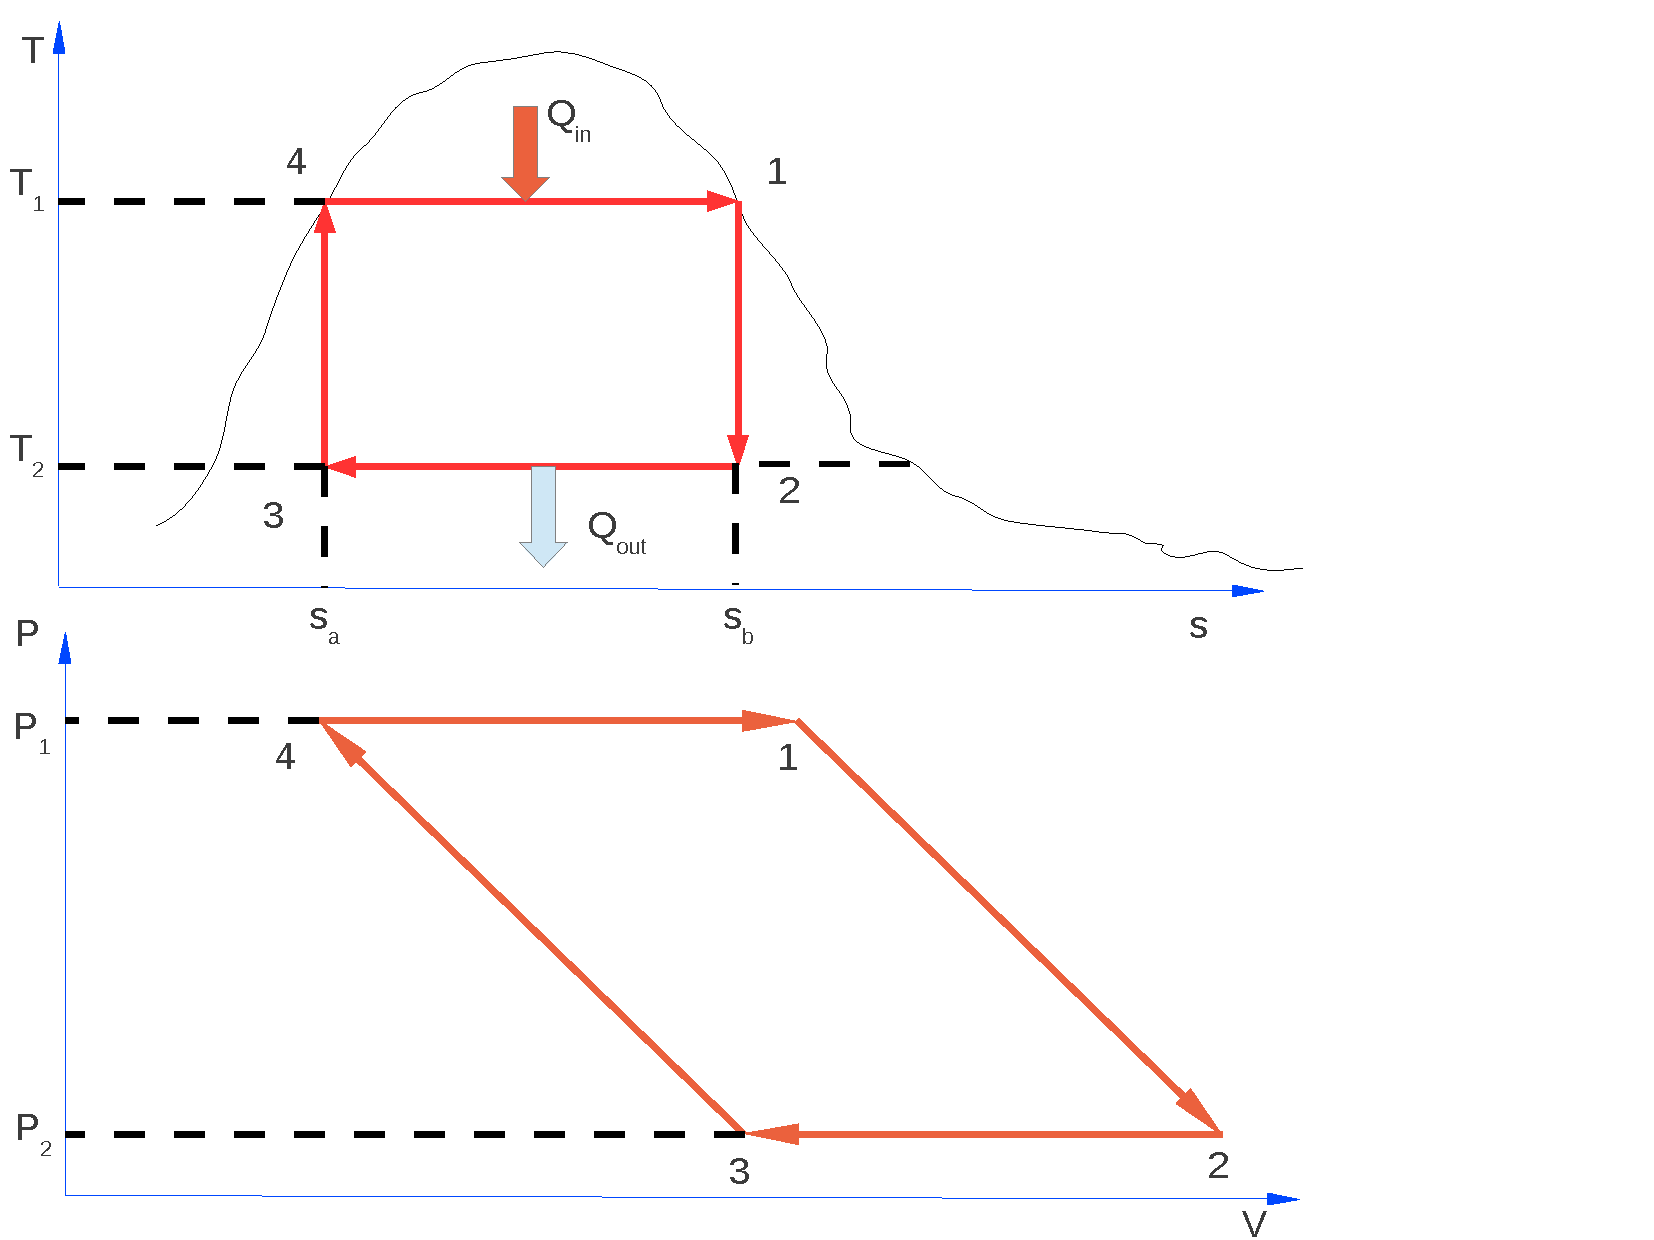
\includegraphics[width=12.cm,clip]{./Pics/Carnot_PV_TS}
    \end{center}
    \caption{Ts and Pv diagrams for Carnot cycle.}\label{PVTSDiags}
   \end{figure}    

%%%
%%% Problem 8.3 (SM&VN)
%%%
%\item {\it A steam power plant operates on the cycle of Fig. \ref{GenericSteamPlant}. For one of the following sets of operating conditions, determine the steam rate, the heat-transfer rates in the boiler and condenser, and the thermal efficiency of the plant.
%\begin{enumerate}
%\item P1 = P2 = 10000 kPa; T2 = 873.15 K; P3 = P4 = 10     kPa; $\eta_{\text{turbine}}$ = 0.80; $\eta_{\text{pump}}$ = 0.75; power rating = 80  MW.
%\item P1 = P2 = 7000  kPa; T2 = 823.15 K; P3 = P4 = 20     kPa; $\eta_{\text{turbine}}$ = 0.75; $\eta_{\text{pump}}$ = 0.75; power rating = 100 MW.
%\item P1 = Pz = 8500  kPa; T2 = 873.15 K; P3 = P4 = 10     kPa; $\eta_{\text{turbine}}$ = 0.80; $\eta_{\text{pump}}$ = 0.80; power rating = 70  MW.
%\item PI = P2 = 6500  kPa; T2 = 798.15 K; P3 = P4 = 101.33 kPa; $\eta_{\text{turbine}}$ = 0.78; $\eta_{\text{pump}}$ = 0.75; power rating = 50  MW.
%\item P1 = P2 = 7760  kPa; T2 = 866.15 K; P3 = P4 = 7      kPa; $\eta_{\text{turbine}}$ = 0.80; $\eta_{\text{pump}}$ = 0.75; power rating = 80  MW.
%\end{enumerate}
%}
%   \begin{figure}[h]
%    \begin{center}
%     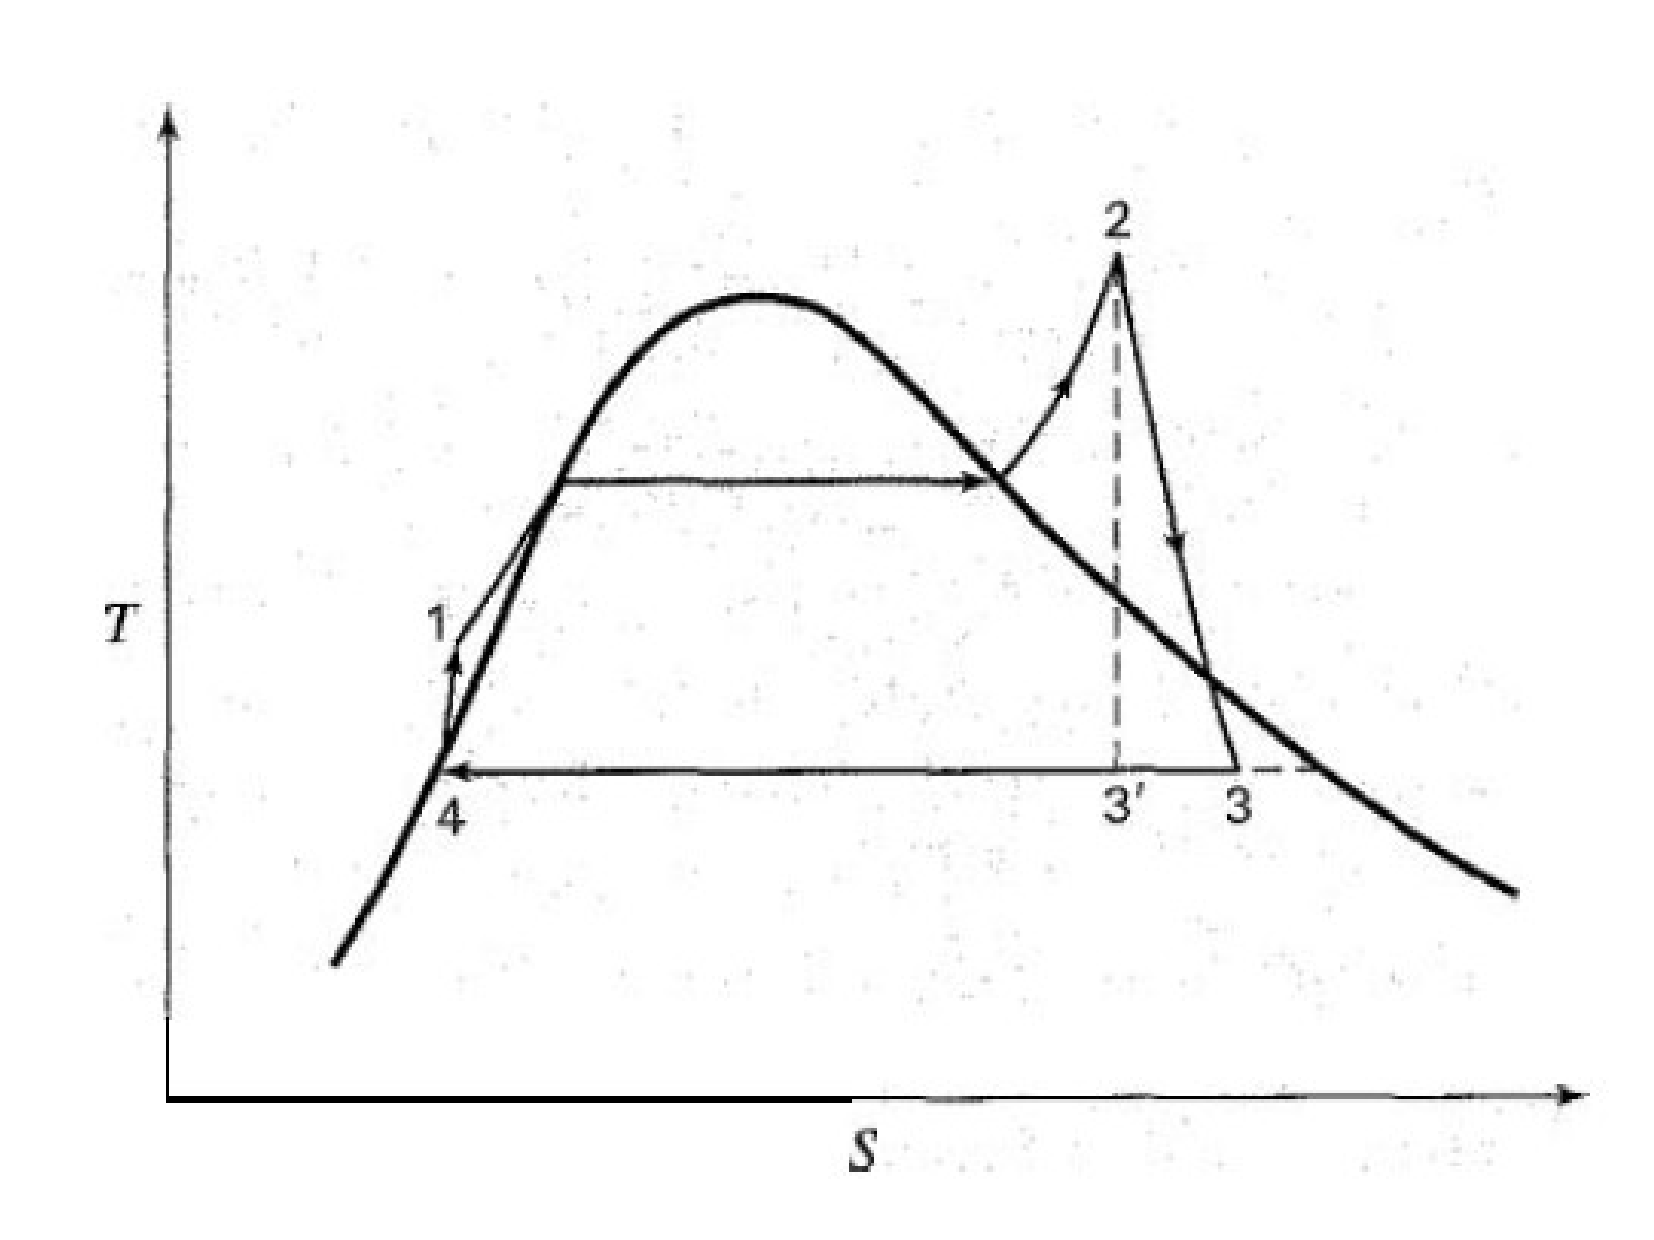
\includegraphics[width=12.cm,clip]{./Pics/Generic_Steam_Cycle}
%    \end{center}
%    \caption{Generic steam power plant.}\label{GenericSteamPlant}
%     \end{figure}

%%%
%%% Example 12.25 (Rajput)
%%%
\item\label{P:example12_25} {\it A steam power plant operates with with regenerative and reheat arrangement cycles. Steam is supplied to the H.P. turbine (Fig. \ref{example12_25}a) at 80 bar and 470$^{o}$C.  For feed heating, a part of steam is extracted at 7 bar and remainder of the steam is reheated to 350$^{o}$C in a reheater and then expanded in L.P. turbine down to 0.035 bar. Determine: (a) amount of steam bled-off for feed heating; (b) amount of steam supplied to L.P. turbine; (c) heat supplied to the boiler and reheater; (d) cycle efficiency, and (e) power developed by the system. The steam supplied by the boiler is 50 kg/s.}
   \begin{figure}[h]
    \begin{center}
    \vbox{
     \hbox{\hspace{1cm}
      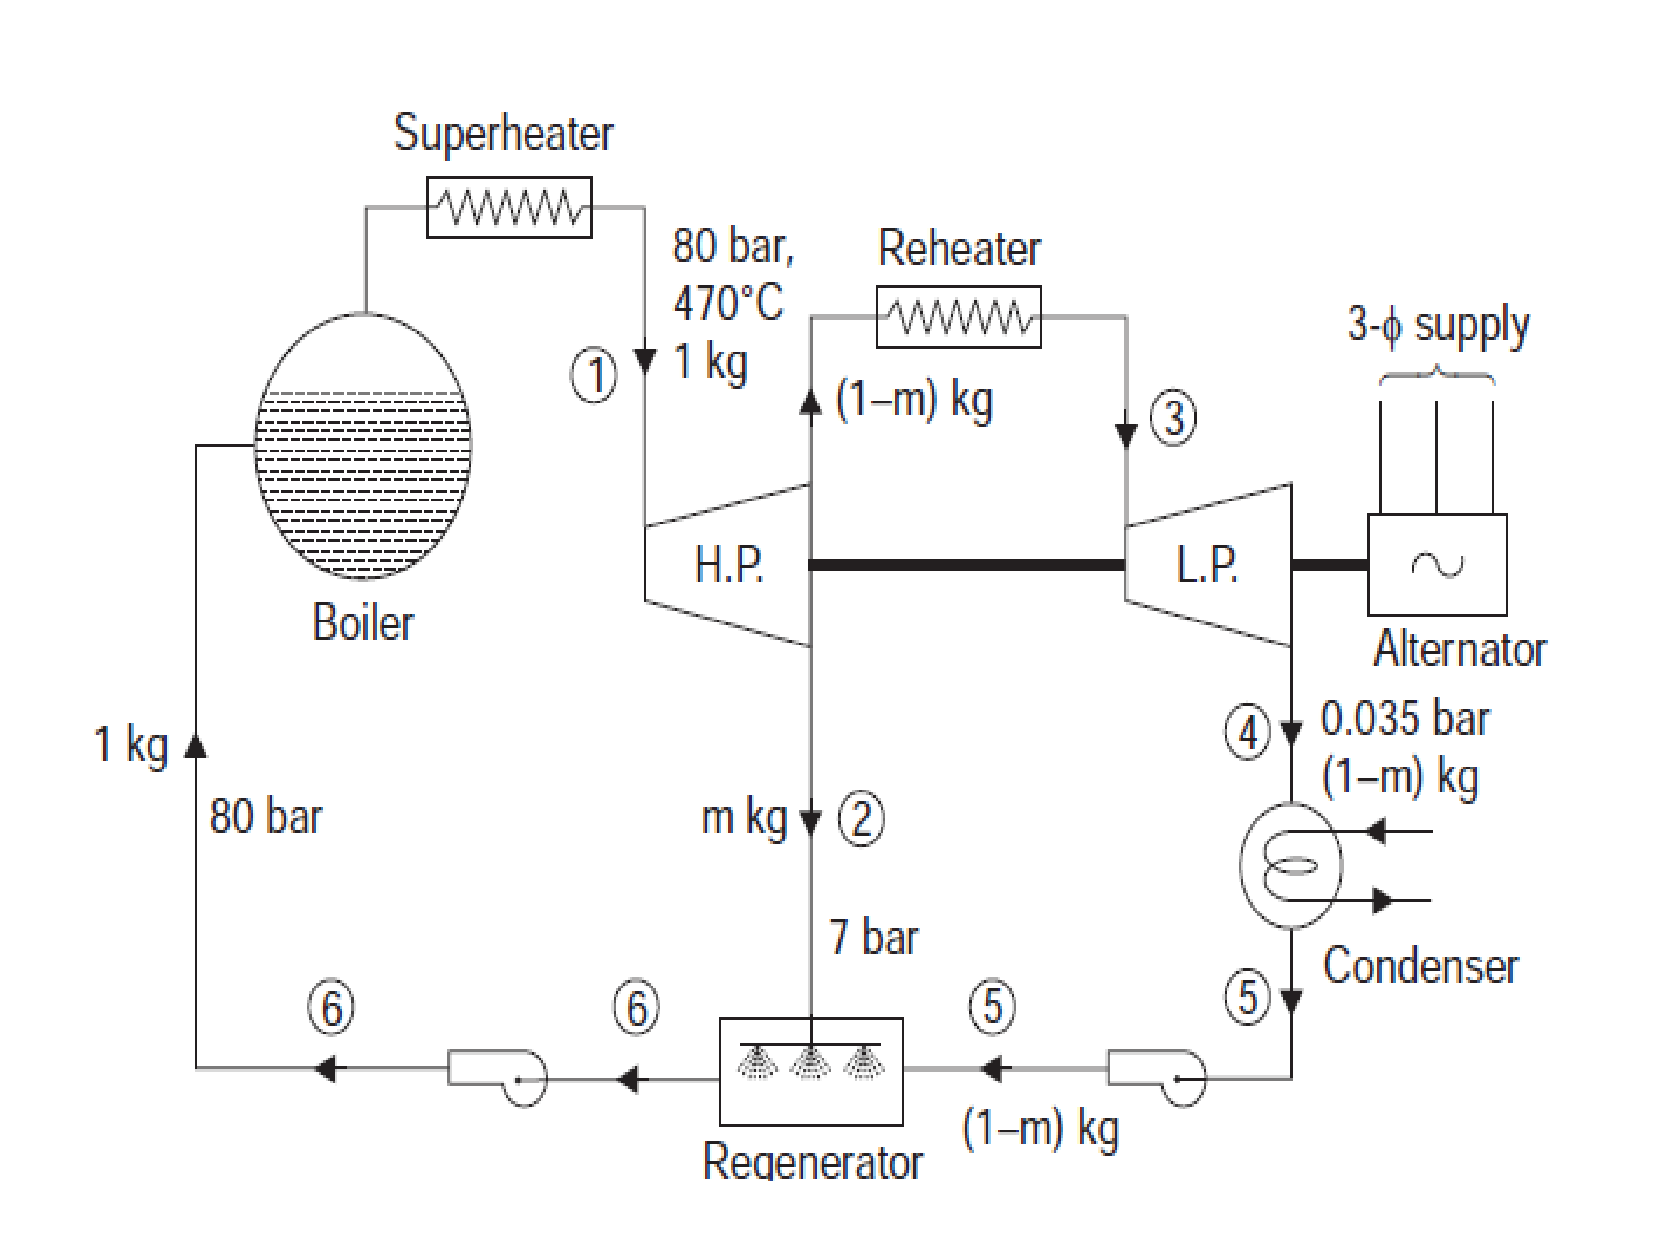
\includegraphics[width=12.cm,clip]{./Pics/Exemple12_25a_Rajput}}
     \hbox{\hspace{7.5cm}(a)}
     \hbox{\hspace{1.cm}
      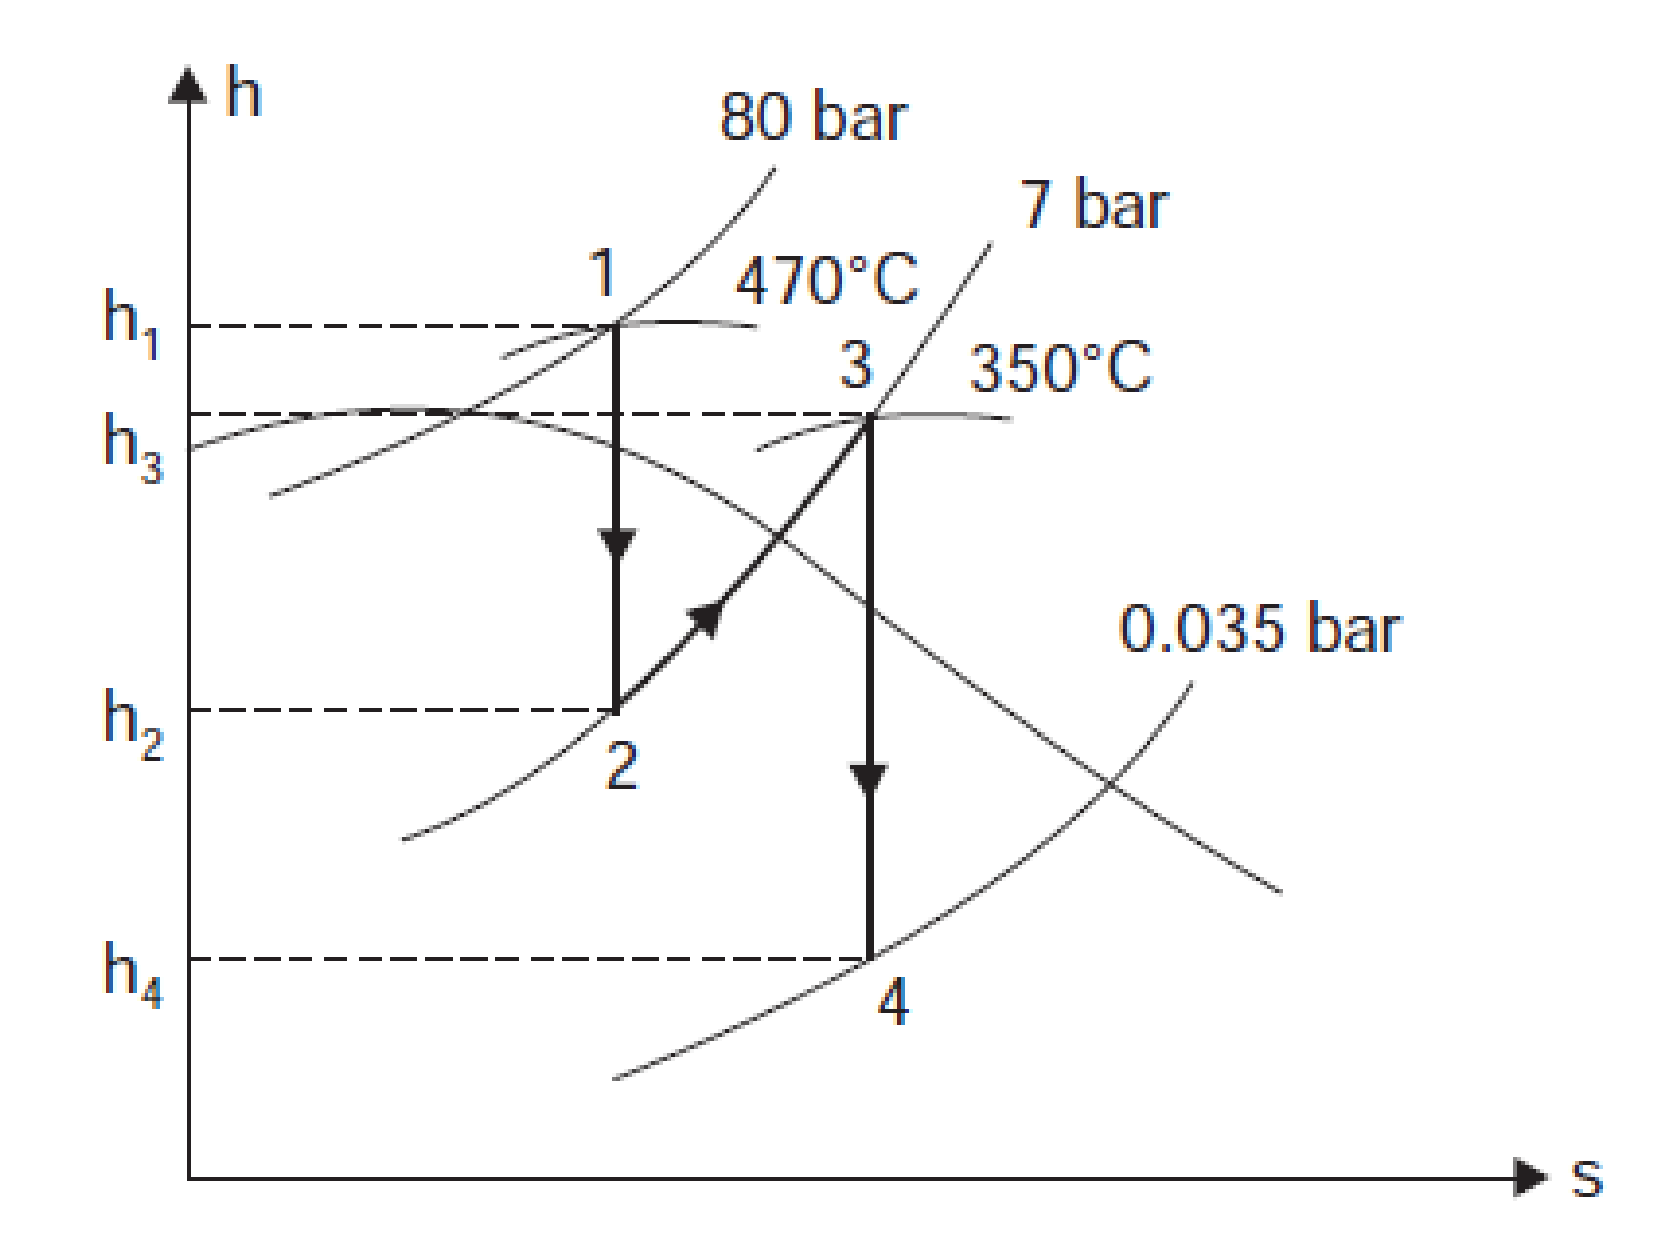
\includegraphics[width=12.cm,clip]{./Pics/Exemple12_25b_Rajput}
      }
     \hbox{\hspace{7.5cm}(b)}}
     \caption{Problem \ref{P:example12_25}: (a) Schematics and (b) $hs$ diagram of a steam power cycle.}
     \label{example12_25}
     \end{center}
   \end{figure}
 

%%%
%%% Problem 8.6 (Saphiro)
%%%
\item {\it Water is the working fluid in an ideal Rankine cycle. Saturated vapour enters the turbine at 16 MPa, and the condenser pressure is 8 kPa. The mass flow rate of steam entering in the turbine is 120 kg/s. Calculate:
\begin{enumerate}
\item the net power developed (in MW);
\item rate of heat transfer to the steam passing through the boiler (in MW);
\item thermal efficiency;
\item mass flow rate of the condenser cooling water (in kg/s(, if the cooling water undergoes a temperature increase of 18$^{o}$C with negligible pressure change in passing through the condenser.
\end{enumerate} 
}


%%%
%%% Problem 8.12 (Saphiro)
%%%
\item {\it A power plant based on the Rankine cycle is under development to provide a net power output of 10MW. Solar collectors are to be used to generate Refrigerant 22 vapour at 1.6MPa and 50$^{o}$C, for expansion through the turbine. Cooling water is available ar 20$^{o}$C. Specify he preliminary design of the cycle and estimate the thermal efficiency and the refrigerant and cooling water flow rates (in kg/s).}



%%%
%%% Problem 8.16 (Saphiro)
%%%
\item {\it Steam enters the turbine of a simple vapour power plant with a pressure of 10 MPa and temperature $T$, and expands adiabatically to 6 KPa. The isentropuc turbine efficiency is 85$\%$. Saturated liquid exits the condenser at 6KPa and the isentropic pump efficiency is 82$\%$.
\begin{enumerate}
\item For $T=580^{o}$C, determine the turbine exit quality and the cycle thermal efficiency;
\item Compute the same of (a) for $T=700^{o}$C.
\end{enumerate}
}





%%%
%%% Problem 8.6 (SM&VN)
%%%
%\item {\it A steam power plant employs two adiabatic turbines in series. Steam enters the first turbine at 650$^{o}\text{C}$ and 7000 kPa and discharges from the second turbine at 20 kPa. The system is designed for equal power outputs from the two turbines, based on a turbine efficiency of 78$\%$ for each turbine. Determine the temperature and pressure of the steam in its intermediate state between the two turbines. What is the overall efficiency of the two turbines together with respect to isentropic expansion of the steam from the initial to the final state? }

%%%
%%% Problem 8.14 (Saphiro)
%%%
%\item \label{P:problem_lava}{\it On the south coast of the island of Hawaii, lava flows continuously into the ocean. It is proposed to anchor a floating power plant off-shore of the lava flow that uses ammonia as the working fluid. The plant would exploit the temperature variation between the warm water near the surface at 130$^{o}$F and seawater at 50$^{o}$F from a depth of 500 ft to produce power. Figure \ref{problem_lava} shows the configuration and provides additional data. Using the properties of pure water for the seawater and modelling the power as a Rankine cycle, calculate: (a) the thermal efficiency; (b) the mass flow rate of ammonia (in kg/h) for a net output of 300 HP.}
%   \begin{figure}[h]
%    \begin{center}
%      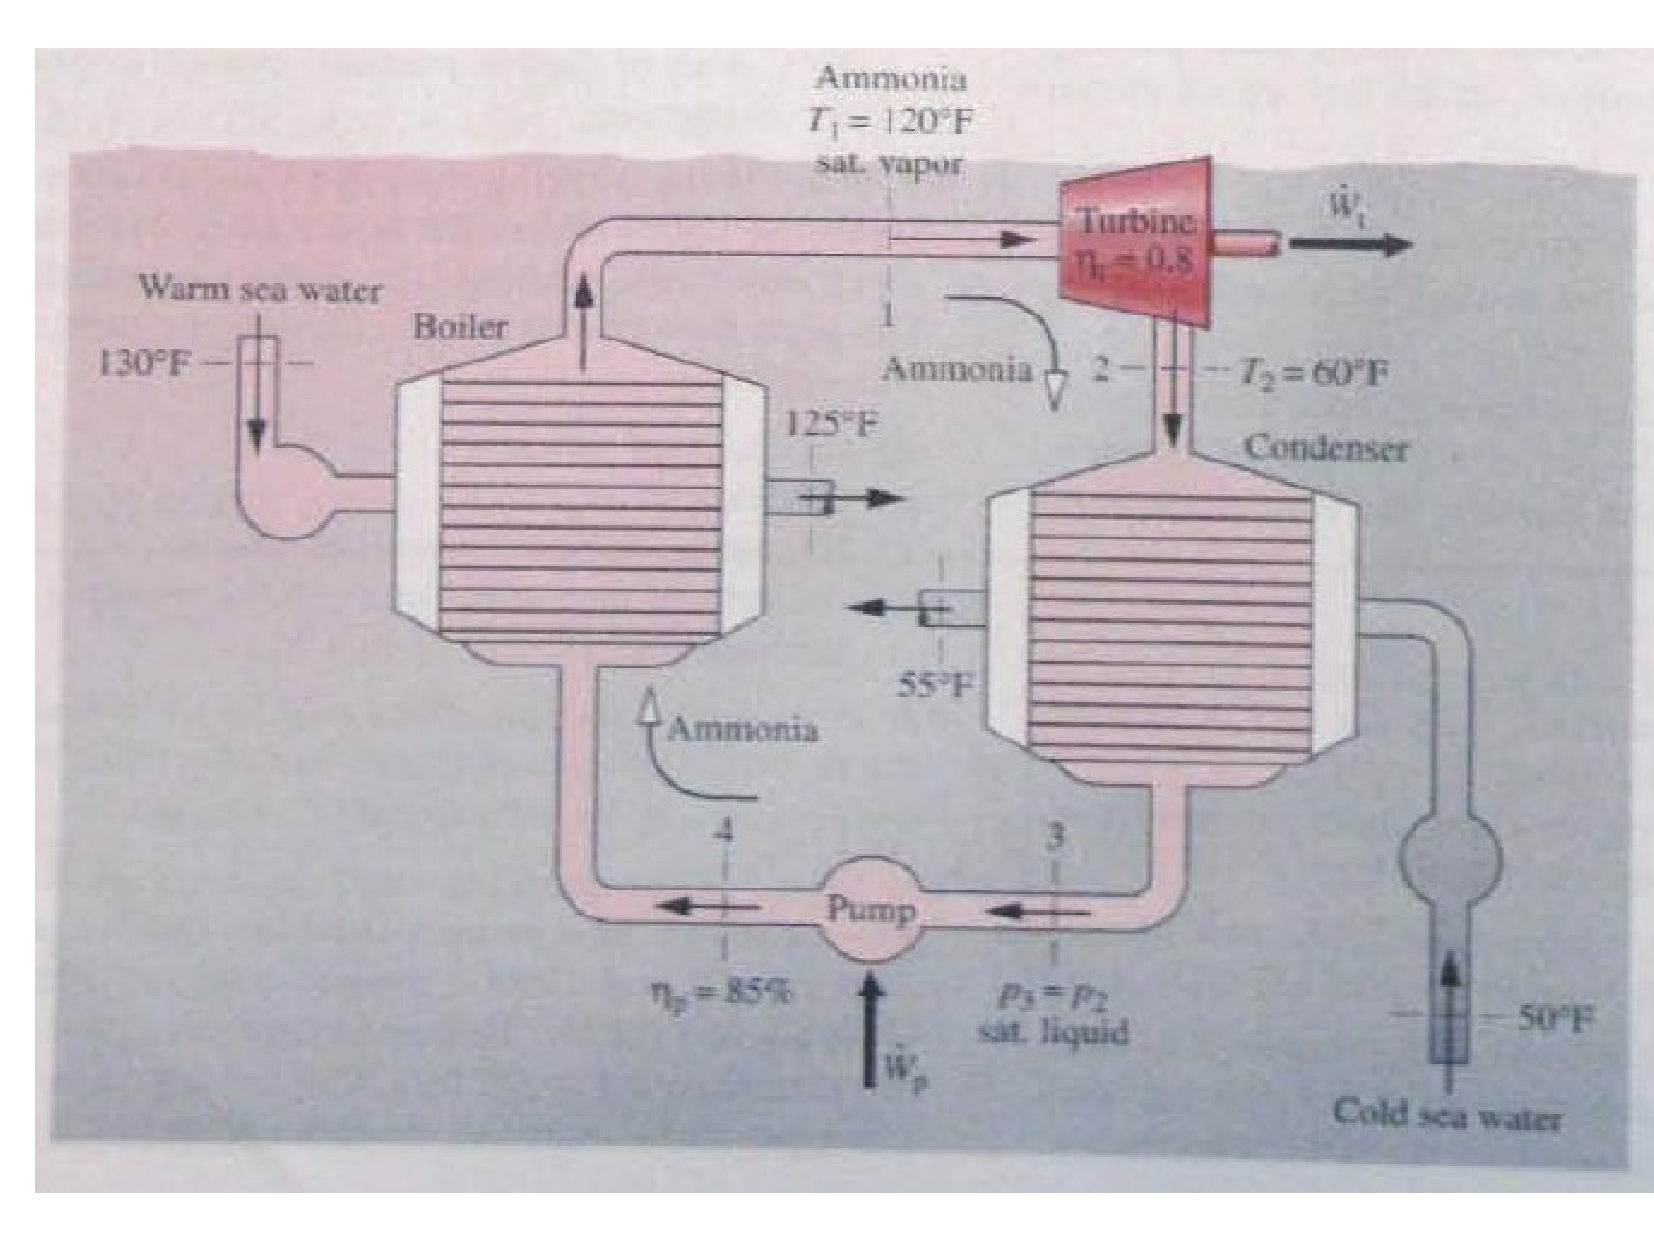
\includegraphics[width=12.cm,clip]{./Pics/LavaVolcanoPlant}
%     \caption{Problem \ref{P:problem_lava}: Schematics a steam power cycle.}
%     \label{problem_lava}
%     \end{center}
%   \end{figure}


%%%
%%% Problem 8.33 (Saphiro)
%%%
\item {\it Steam at 32 MPa and 520$^{o}$C enters the first stage of a supercritical reheat cycle including three turbine stages. Steam exiting the first-stage turbine at pressure $P$ is reheated at constant pressure to 440$^{o}$C, and steam exiting the second-stage turbine at 0.5 MPa is reheated at constant pressure to 360$^{o}$C.  Each turbine stage and the pump has an isentropic effciency of 85$\%$. The condenser pressure is at 8 kPa. For $P=4\;MPa$, determine the net work per unit mass of steam flowing (kJ/kg) and the thermal efficiency.}


%%%
%%% Problem 8.9 (SM&VN). \ref{example8_9})
%%%
\item \label{P:example8_9}{\it Steam power plant operating on a regenerative cycle, includes just one feedwater heater. Steam enters the turbine at 4500 kPa and 773.15 K and exhausts at 20 kPa. Steam for the feedwater heater is extracted from the turbine at 350 kPa, and in condensing raises the temperature of the feedwater to within 6 K of its condensation temperature at 350 kPa. If the turbine and pump efficiencies are both 0.78, what is the thermal efficiency of the cycle and what fraction of the steam entering the turbine is extracted for the feedwater heater?}



%\item \label{P:example8_9}{\it A steam power plant operating on a regenerative cycle (Fig. \ref{example8_9}), includes two feedwater heaters. Steam enters the turbine at 6500 kPa and 873.15 K and exhausts at 20 kPa. Steam for the feedwater heaters is extracted from the turbine at pressures such that the feedwater is heated to 463.15 K in two equal increments of temperature rise, with 5 K approaches to the steam-condensation temperature in each feedwater heater. If the turbine and pump efficiencies are both 0.80, what is the thermal efficiency of the cycle and what fraction of the steam entering the turbine is extracted for each feedwater heater? }


%\item \label{P:example8_10}{\it A power plant operating on heat recovered from the exhaust gases of internal combustion engines uses isobutane as the working medium in a modified Rankine cycle in which the upper pressure level is above the critical pressure of isobutane. Thus the isobutane does not undergo a change of phase as it absorbs heat prior to its entry into the turbine. Isobutane vapour is heated at 4800 kPa to 533.15 K, and enters the turbine as a supercritical fluid at these conditions. Isentropic expansion in the turbine produces a superheated vapour at 450 kPa, which is cooled and condensed at constant pressure. The resulting saturated liquid enters the pump for return to the heater. If the power output of the modified Rankine cycle is 1000 kW, what is the isobutane flow rate, the heat-transfer rates in the heater and condenser, and the thermal efficiency of the cycle? The vapour pressure of isobutane is given by
%\begin{displaymath}
%\ln\left(P^{\text{sat}}\right) = 1 - \frc{2606.775}{T+0.918}\;\;\;\text{with}\;\;\;\left[P^{\text{sat}}\right]=\text{kPa}\;\;\;\text{and}\;\;\;\left[T\right]=\text{K}
%\end{displaymath}
%Also, the enthalpy of the liquid flows can be obtained from
%\begin{displaymath}
%\Delta H = C_{p}\Delta T + V\left(1-\beta T\right)\Delta P
%\end{displaymath} 
%where
%\begin{displaymath}
%\beta=\frc{1}{V}\left(\frc{\partial V}{\partial T}\right)_{P}
%\end{displaymath}
%is the volume expansivity of fluid.
%}


   %\begin{figure}[h]
   % \begin{center}
   %   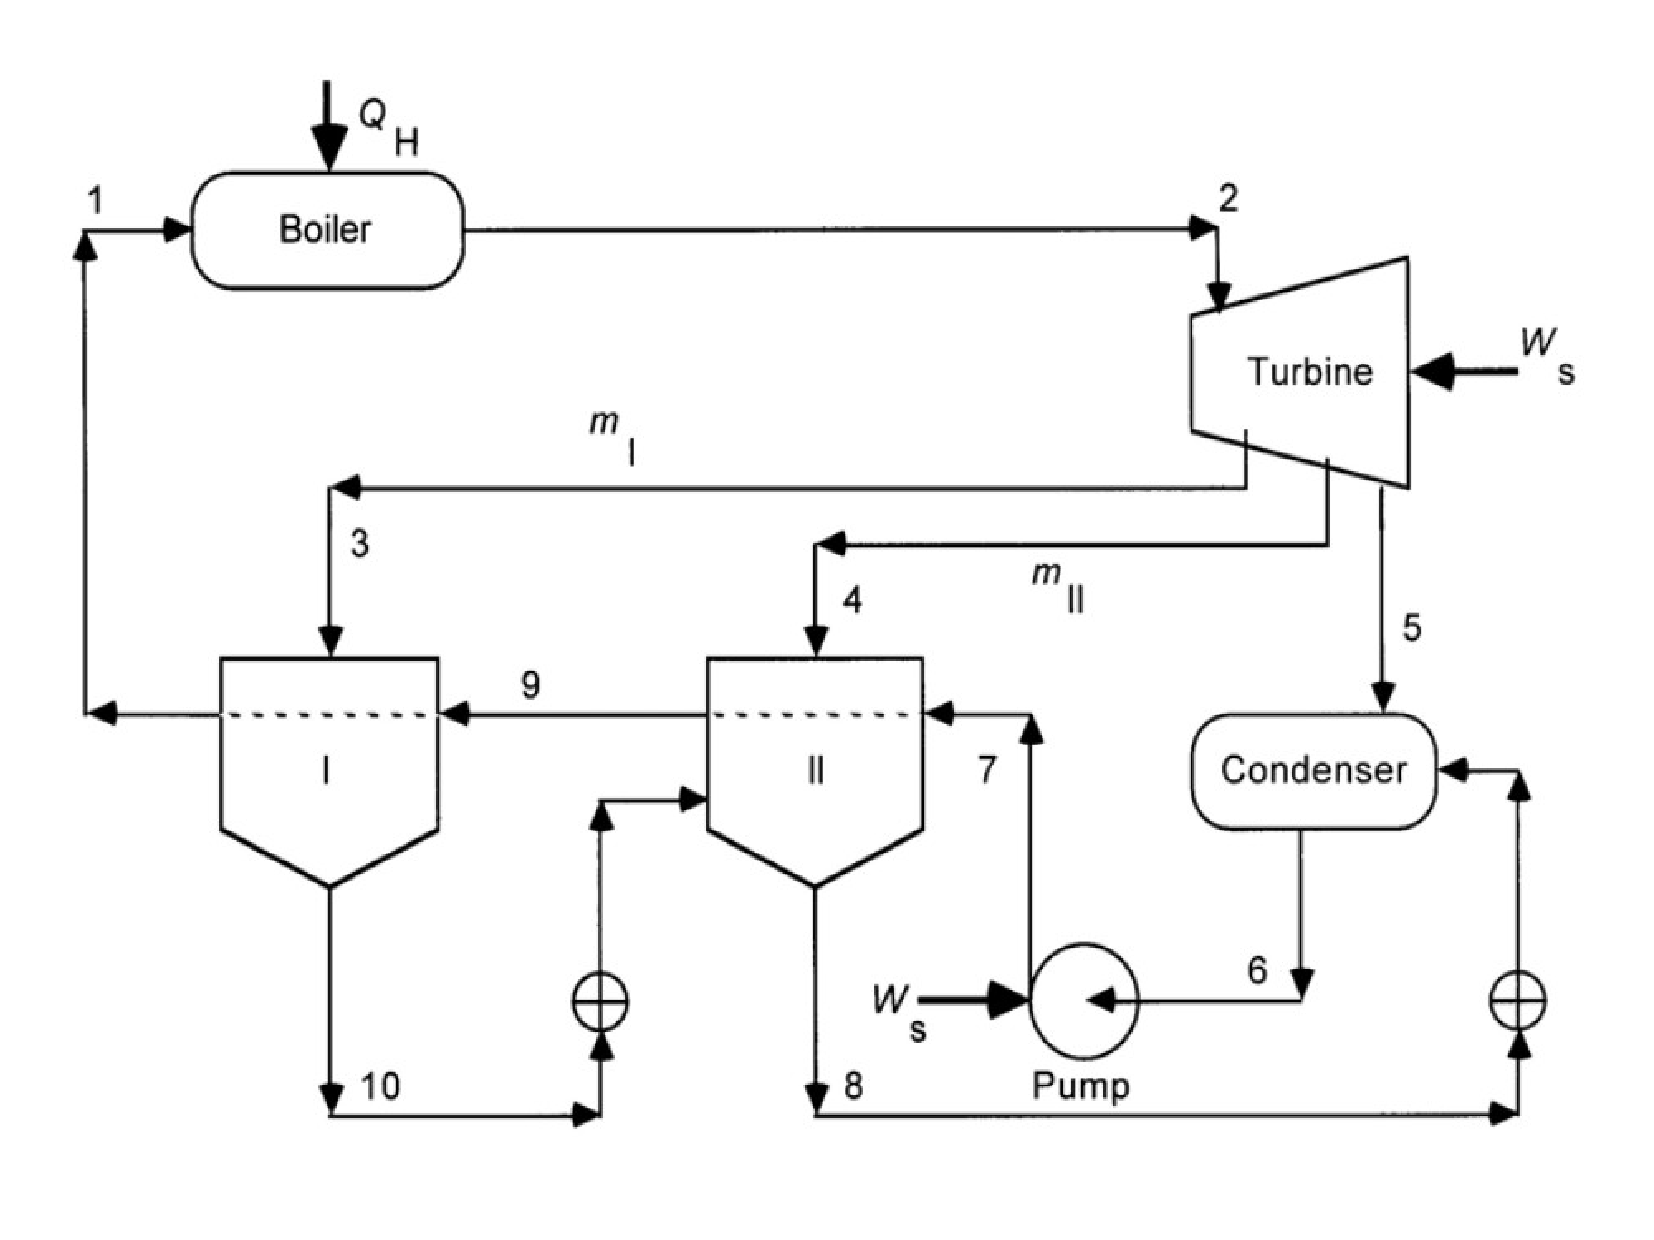
\includegraphics[width=12.cm,clip]{./Pics/Example_SMVN_8_9}
   %  \caption{Problem \ref{P:example8_9}: Schematics modified Rankine power cycle.}
   %  \label{example8_9}
   %  \end{center}
   %\end{figure}
 


%%%
%%% Problem 8.10 (SM&VN)
%%%
%\item {\it A power plant operating on heat from a geothermal source uses isobutane as the working medium in a Rankine cycle (Fig.\ref{GenericSteamPlant}). Isobutane is heated at 4.8 MPa (a pressure just below its critical pressure) to a temperature of 533.15 K, at which conditions it enters the turbine. Isentropic expansion in the turbine produces superheated vapour at 450 kPa, which is cooled and condensed to saturated liquid and pumped to the heater/boiler. If the flow rate of isobutane is 75 kg/s, what is the power output of the Rankine cycle and what are the heat-transfer rates in the heater/boiler and cooler/condenser? What is the thermal efficiency of the cycle? Repeat these calculations for a cycle in which the turbine and pump each have an efficiency of 80$\%$. The vapour pressure of isobutane is given in Problem \ref{P:example8_9}.}



\end{enumerate}


